\chapter{Théorèmes de Pythagore et Thalès}

\section{Pythagore}

Ce chapitre s'intéresse à l'un des théorèmes les plus connus dans la population : le théorème de Pythagore.

\subsection{Un peu d'histoire}

Pythagore\index{Pythagore} est né 580 ans avant notre ère, en Grèce. C'est une période  faste pour la classe supérieure de la société. La médecine fait beaucoup de progrès, la vie devient moins pénible grâce au travail de nombreux esclaves qui s'occupent des tâches difficiles. La culture grecque rayonne dans toute l'Europe. Les savants voyagent, échangent avec des personnes d'autres cultures (égyptienne, babylonienne, indienne) et s'intéressent à la philosophie et aux mathématiques. C'est une gymnastique mentale, mais aussi une réflexion sur l'existence, le bonheur, l'amour, etc.

Pythagore fait partie de cette classe privilégiée, parcourt le monde (c'est-à-dire, à l'époque, le bassin méditerranéen) et étudie les textes d'autres civilisations. Il s'intéresse beaucoup aux nombres et fonde une école de pensée, l'école pythagoricienne, qui tente d'expliquer le monde par les nombres.

Il serait faux de voir cette école comme l'on se représente actuellement un salle de classe. A l'époque, ce courant de pensée s'apparentait plus à une secte : différents grades selon la compréhension des nombres, des rites de passages pour le grade supérieur, un enseignement où le maître se cachait derrière un rideau.

C'est dans ces conditions que Pythagore met en lumière une relation dans les triangles rectangles, mais qui était déjà connue des Babyloniens en -3000. Le lien aux nombres est tellement fort dans cette école que quand Aristote, un autre philosophe de la même époque, démontre que l'hypoténuse d'un triangle rectangle ayant chacune de ses cathètes de longueur 1 ne peut pas être une fraction, le choc est si grand (il existe des nombres qui ne sont pas des fractions) qu'une partie des Pythagoriciens se suicide.

\subsection{Et un peu de math}

\begin{definition}
Un triangle rectangle est un polygone formé de trois côtés : l'hypoténuse (du grec hypo-tenuse, sous-tenu) et de deux cathètes de manière à ce que ces dernières forment un angle droit. 
\end{definition}

\begin{notation}
Les trois sommets sont appelés $A$, $B$ et $C$, toujours notés dans le sens contraire des aiguilles d'une montre, les trois côtés sont appelés $a$, $b$ et $c$ selon le sommet qui leur fait face et les trois angles $\alpha $, $\beta $ et $\gamma $ selon le sommet auquel ils appartiennent.

\begin{center}
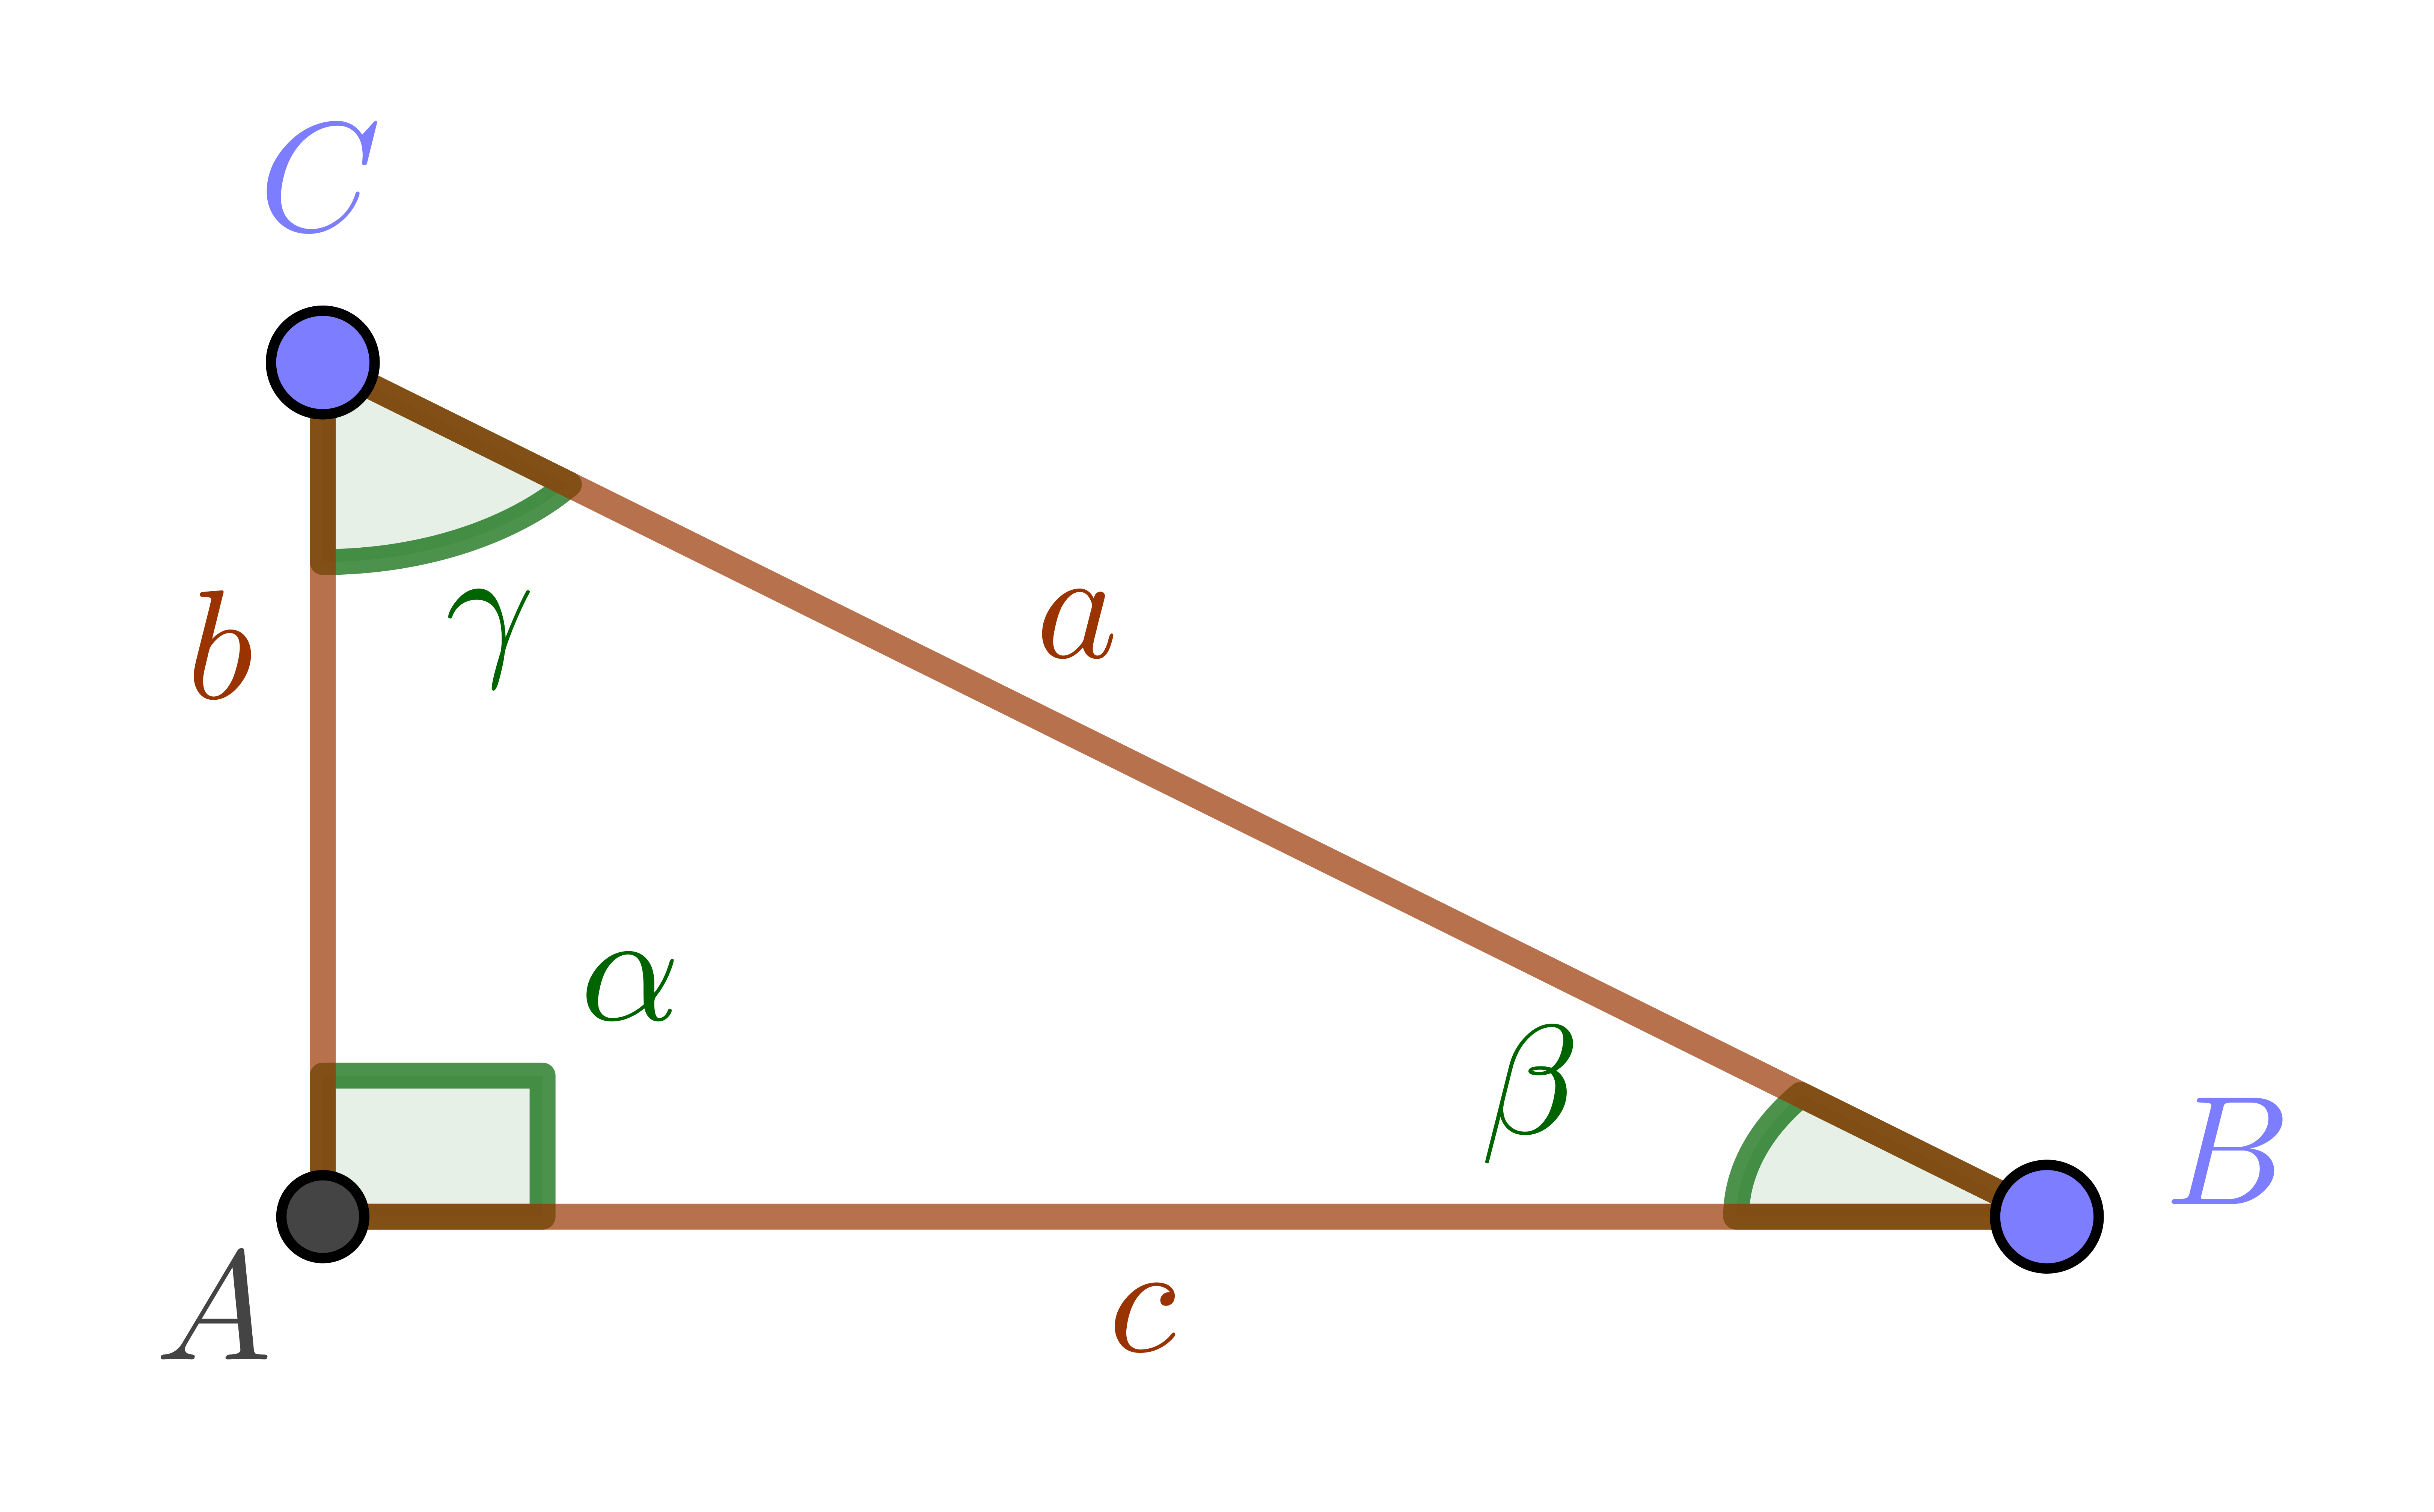
\includegraphics[width=0.4\textwidth]{triangle/image/triangle.png}
\end{center}
\end{notation}

Le théorème de Pythagore fait le lien entre les trois côtés d'un triangle rectangle.

\begin{theoreme}
Dans un triangle rectangle, le carrés de l'hypoténuse est égale à la somme des carré des cathètes.
\end{theoreme}

\begin{center}
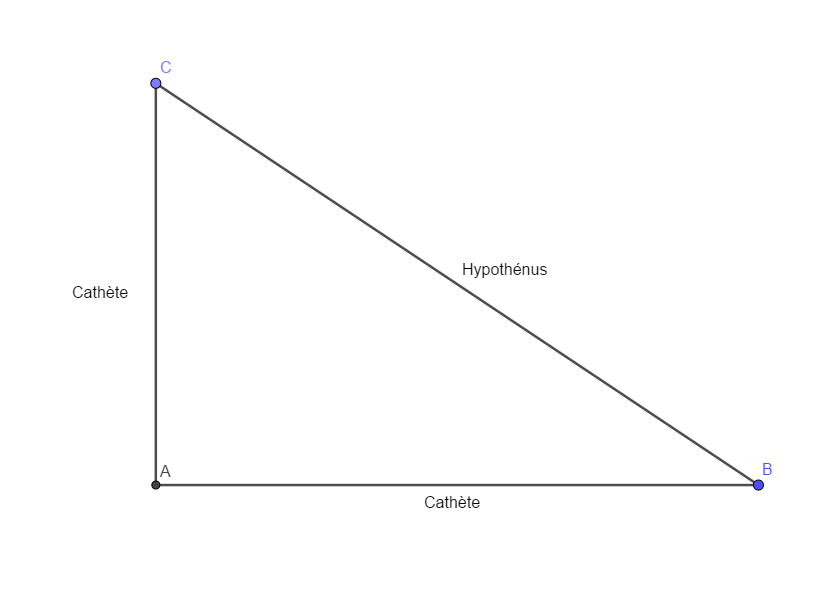
\includegraphics[width=0.9\textwidth]{triangle/image/pythagore.png}
\end{center}

\section{Thalès}

Thalès de Milet, s'il est moins connu que Pythagore, est aussi un philosophe et un mathématicien de la Grèce antique. Ses dates de naissance et de mort sont plus floues, mais on estime qu'il a vécu à la même époque que Pythagore.

Il a repris certaines propriétés géométriques du plan vraisemblablement connues des Égyptiens, mais en a fait une théorie abstraite. Il est un peu le père des figures parfaites : par exemple en vrai on ne peut pas dessiner une droite, car une droite n'a pas d'épaisseur. Cependant, on peut considérer que la représentation qu'on a faite de la droite comme suffisamment proche de la droite parfaite.

\begin{definition}
Deux triangles sont dits \emph{semblables} si leurs trois côtés sont sur des droites parallèles.
\end{definition}

La grande idée de Thalès est de remarquer que des triangles semblables ne diffèrent que par leur échelle, ainsi les proportions sont préservées.

\begin{theoreme}
Dans deux triangles semblables, les rapports des côtés sont les mêmes. Par exemple, pour les triangles $ABC$ et $A'B'C'$, on a :
$$
\frac{a}{b} = \frac{a'}{b'}\hspace{1cm} \frac{a}{c} = \frac{a'}{c'} \hspace{1cm} \frac{b}{c} = \frac{b'}{c'}
$$
ou
$$
\frac{a}{a'} = \frac{b}{b'} = \frac{c}{c'} = \mbox{ coefficient d'homothétie}
$$
\end{theoreme}

\begin{center}
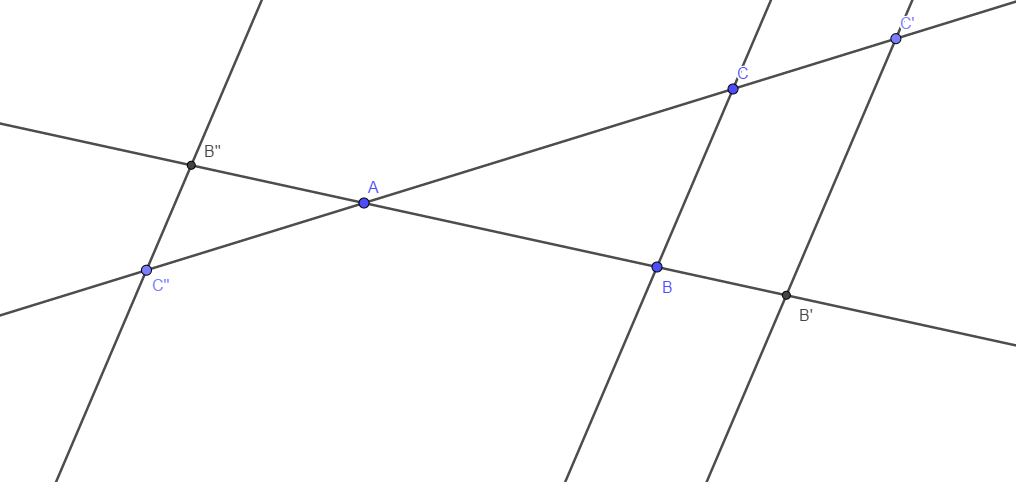
\includegraphics[width=0.9\textwidth]{triangle/image/thales.png}
\end{center}

\section{Exercices}

\begin{exercice}
Dans un triangle rectangle, l'hypoténuse mesure 50 cm et l'une des cathètes 48 cm.
Quelle est la mesure de l'autre cathète ?
\end{exercice}

\begin{exercice}
Es-tu en présence de triangles rectangles ?

\begin{center}
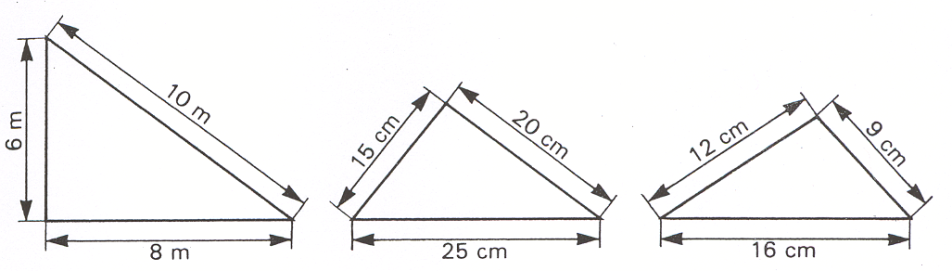
\includegraphics[width = 0.4 \textwidth]{triangle/image/pyth2.png}
\end{center}



\end{exercice}

\begin{exercice}
Calculer l'aire du rectangle dont la diagonale mesure 125 cm et la largeur 44 cm.

\end{exercice}

\begin{exercice}
L'aire d'un triangle isocèle abc ($\overline{ab}=\overline{ac}$) mesure 2640 cm2. La hauteur abaissée du sommet a sur le côté [bc] mesure 55 cm.
Calculer le périmètre du triangle abc.

\end{exercice}

\begin{exercice}
Quelle est l'aire d'un losange dont le périmètre mesure 260 cm et l'une des diagonales 66 cm ?

\end{exercice}

\begin{exercice}
Dans un trapèze rectangle, la petite base vaut les 8/11 de la grande base. Sachant que la hauteur du trapèze mesure 1,2 m et l'aire 4,788 m2, calculer le périmètre du trapèze.

\end{exercice}

\begin{exercice}
Calculer l'aire tramée sachant que les cathètes [ab] et [ac] mesurent respectivement 28 cm et 45 cm.
\begin{center}
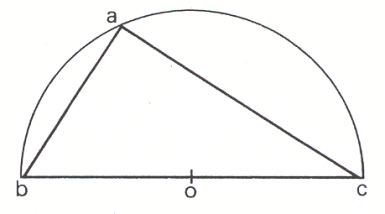
\includegraphics[width = 0.4 \textwidth]{triangle/image/pyth7.png}
\end{center}
\end{exercice}

\begin{exercice}
Les bases d'un trapèze isocèle mesurent 45 cm et 62 cm.
Le périmètre du trapèze est égal à 153 cm. Calculer :
l'aire de ce trapèze;
la longueur d'une des diagonales.

\end{exercice}

\begin{exercice}
La corde [ab] mesure 2 m et est parallèle au diamètre [cd] dont la mesure est 3 m.
Quelle distance sépare ces deux droites ?
\begin{center}
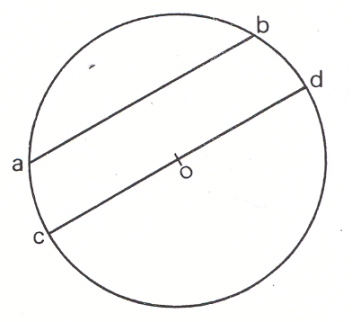
\includegraphics[width = 0.4 \textwidth]{triangle/image/pyth9.png}
\end{center}
\end{exercice}

\begin{exercice}
Calculer l'aire et le périmètre d'un carré inscrit dans un cercle de 12 cm de rayon.

\end{exercice}

\begin{exercice}
Un cercle est inscrit dans un carré dont la diagonale mesure 24 cm.
Quelle est l'aire de la surface comprise entre le carré et le cercle ?

\end{exercice}

\begin{exercice}
Les triangles aed, fgh et ijk sont isocèles.
Sachant que $\overline{ik}=2\text{ cm }\cdot \text{ }\sqrt{\text{2}}$, calculer la longueur de côté [ad].
\begin{center}
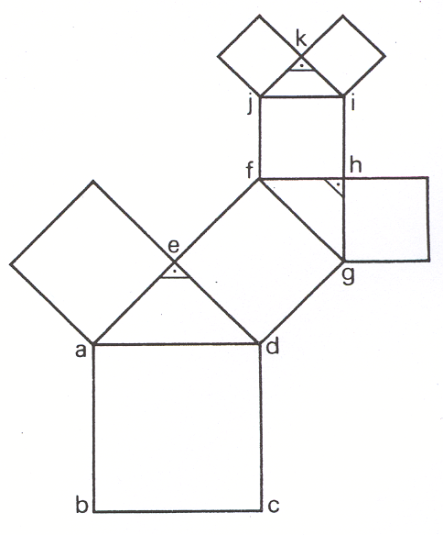
\includegraphics[width = 0.4 \textwidth]{triangle/image/pyth12.png}
\end{center}
\end{exercice}

\begin{exercice}
Quelle est l'aire d'un triangle équilatéral dont le côté mesure 18 cm ?


\end{exercice}

\begin{exercice}
Sachant que : $\overline{ah}=13,2\text{ cm , }\overline{\text{ad}}=\text{ 27,5 cm et }\overline{\text{ac}}\text{ = 22 cm}$
Calculer le périmètre du parallélogramme abcd.
\begin{center}
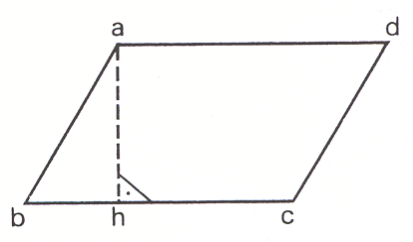
\includegraphics[width = 0.4 \textwidth]{triangle/image/pyth14.png}
\end{center}
\end{exercice}

\begin{exercice}
Un octogone régulier dont le côté mesure 15,3 cm est inscrit dans un cercle de 20 cm de rayon.
Quelle est l'aire de la surface comprise entre le cercle et l'octogone ?


\end{exercice}

\begin{exercice}
Sachant que $\overline{ac}=\text{ 77 cm et }\overline{\text{bc}}\text{ = 85 cm}$,
calculer l'aire de la surface tramée et compare-la à celle du triangle rectangle.
\begin{center}
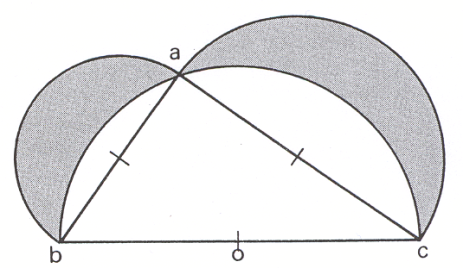
\includegraphics[width = 0.4 \textwidth]{triangle/image/pyth16.png}
\end{center}
\end{exercice}

\begin{exercice}
On dit qu'un homme aurait imaginé que la Terre était ronde en voyant revenir au port un vaisseau qu'il avait observé à la longue-vue quelques jours auparavant. Le vaisseau gagnait alors le large et cette personne le vit prendre l'eau puis disparaître complètement dans la mer. Admettons que la pointe du mât culminait à 20 m au-dessus des flots et que la longue-vue se trouvait à 2 m d'altitude au moment de l'observation.
Quelle était alors la distance entre le vaisseau et l'observateur lorsque ce dernier vit disparaître la pointe du mât ? 
(Prendre 6'400 km pour le rayon de la Terre).
\begin{center}
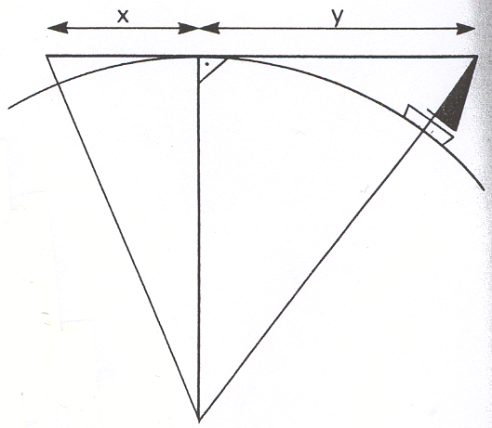
\includegraphics[width = 0.4 \textwidth]{triangle/image/pyth17.png}
\end{center}
\end{exercice}

\begin{exercice}
Soit le triangle abc tel que $\overline{ab}=\text{ 3 dm, }\overline{\text{bc}}\text{ = 6 dm et }\overline{\text{ac}}\text{ = 4 dm}$.
On mène parallèlement au côté [bc] une droite qui coupe [ab] en d et [ac] en e telle que $\overline{de}=\overline{\text{ac}}\text{ }$.
Calculer $\overline{ad}\text{ }et\text{ }\overline{\text{ec}}\text{ }$.


\end{exercice}

\begin{exercice}
Soit un arc de cercle de centre o et de rayon r = 1 cm et un triangle oab rectangle en a.
Le point b' est l'intersection de l'arc de cercle et de l'hypoténuse.
On mène par b' une parallèle à [ab]. Sachant que : $\overline{a'b'}\text{ = 0,8 cm }et\text{ }\overline{\text{ob}}\text{ = 17,5 cm, calculer }\overline{\text{oa}}\text{ et }\overline{\text{ab}}.$
\begin{center}
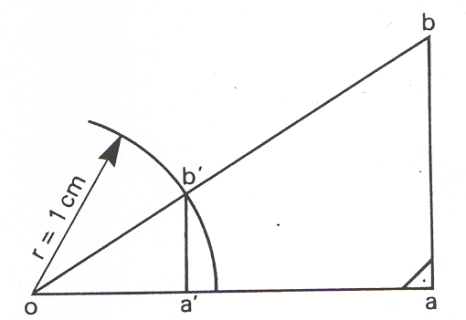
\includegraphics[width = 0.4 \textwidth]{triangle/image/pyth19.png}
\end{center}
\end{exercice}

\begin{exercice}
Soit un arc de cercle de centre o et de rayon r = 1 cm et un triangle oab rectangle en a.
Le point a' est l'intersection de l'arc de cercle et de la cathète [oa].
On mène par a' une parallèle à [ab]. 
Sachant que : $\overline{a'b'}\text{ = 0,72 cm }et\text{ }\overline{\text{ab}}\text{ = 6,12 cm}$, 
calculer le périmètre du triangle abo
\begin{center}
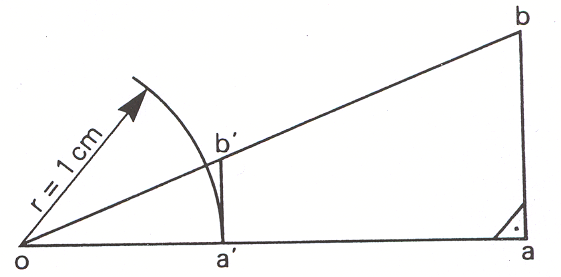
\includegraphics[width = 0.4 \textwidth]{triangle/image/pyth20.png}
\end{center}
\end{exercice}

\begin{exercice}
Soit deux droites sécantes A et B et trois parallèles ad, be, cf.
$\overline{ab}\text{ = 15 cm}$, $\text{ }\overline{\text{ac}}\text{ = 20 cm}$
et $\overline{\text{ef}}\text{ = 8 cm}$.
Calculer la longueur des segments [de] et [df].
\begin{center}
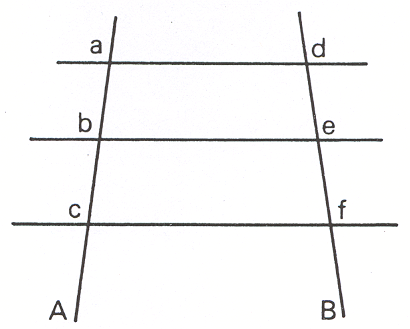
\includegraphics[width = 0.4 \textwidth]{triangle/image/pyth21.png}
\end{center}
\end{exercice}

\begin{exercice}
Les droites parallèles ab, cd, ef, gh coupent les sécantes A et B.
Sachant que : $\overline{ac}\text{ = 15 cm},\text{ }\overline{\text{ag}}\text{ = 60 cm,  }\overline{\text{dh}}\text{ = 72 cm, }\overline{\text{df}}\text{ = 40 cm}$,
Calculer : $\overline{bd},\text{ }\overline{\text{cg}}\text{, }\overline{\text{ce}}\text{, }\overline{\text{eg}}\text{ }$.
\begin{center}
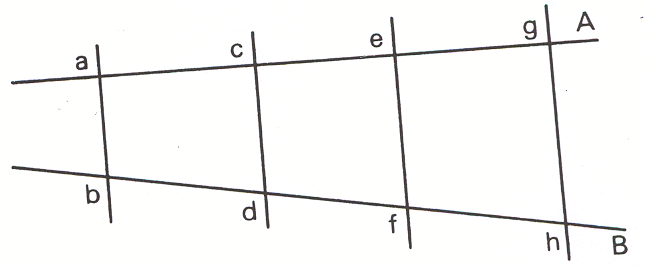
\includegraphics[width = 0.4 \textwidth]{triangle/image/pyth22.png}
\end{center}
\end{exercice}

\begin{exercice}
Soit deux droites sécantes A et B et trois parallèles ab, cd, ef.
On connaît : $\overline{ac}\text{ = 18 cm},\text{ }\overline{\text{ae}}\text{ = 45 cm, }\overline{\text{df}}\text{ = 36 cm}$.
Calculer les longueurs des segments [bd] et [bf].
\begin{center}
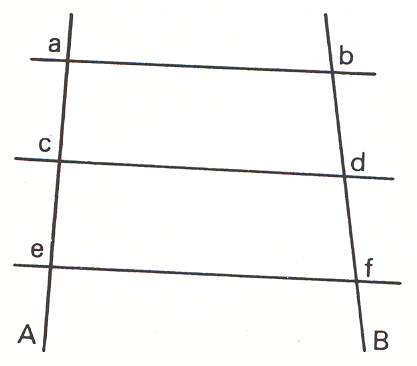
\includegraphics[width = 0.4 \textwidth]{triangle/image/pyth23.png}
\end{center}
\end{exercice}

\begin{exercice}
Calculer le volume d’un tronc de cône haut de 60 cm et dont le diamètre de la grande base mesure 30 cm et celui de la petite 15 cm.


\end{exercice}

\begin{exercice}
Calculer le volume d’une pyramide tronquée à base carrée de 80 mm de côté de la grande base, 25 mm de côté de la petite base et dont la hauteur mesure 45 mm.

\end{exercice}